\documentclass[8pt, twocolumn]{article}
\usepackage[margin=1in]{geometry}
\usepackage{lmodern} % http://ctan.org/pkg/lm
\usepackage{authblk} % adds affiliations

\usepackage[utf8x]{inputenc}
\usepackage{nameref}
\usepackage[switch]{lineno}
\usepackage{amsmath}
\usepackage{mathtools} % for \prescript{} command
\usepackage{booktabs}
\usepackage[numbers,super]{natbib}
\usepackage{changepage}

% for pseudocode
\usepackage[]{algorithm2e}


% adjust caption style
\usepackage[aboveskip=1pt,labelfont=bf,
            labelsep=period,singlelinecheck=off]{caption}

% remove brackets from references
\makeatletter
\renewcommand{\@biblabel}[1]{\quad#1.}
\makeatother

\usepackage[colorinlistoftodos]{todonotes}

% headrule, footrule and page numbers
\usepackage{lastpage,fancyhdr,graphicx}
\usepackage{epstopdf}
\pagestyle{myheadings}
\pagestyle{fancy}
\fancyhf{}
\rfoot{\thepage/\pageref{LastPage}}
\renewcommand{\footrule}{\hrule height 2pt \vspace{2mm}}

% use \textcolor{color}{text} for colored text (e.g. highlight to-do areas)
\usepackage{color}

\definecolor{Gray}{gray}{.25}

\usepackage{graphicx}

% use if you want to put caption to the side of the figure
\usepackage{sidecap}

\usepackage{xcolor}
\usepackage[colorlinks = true,
            linkcolor = blue,
            urlcolor  = blue,
            citecolor = blue,
            anchorcolor = blue]{hyperref}

% ####################################################
% ####################################################
\usepackage[colorinlistoftodos]{todonotes}
% ####################################################
% ####################################################

% use for have text wrap around figures
\usepackage{wrapfig}
\usepackage[pscoord]{eso-pic}
\usepackage[fulladjust]{marginnote}
\reversemarginpar{}

\usepackage{gensymb}
\usepackage{siunitx}

% make a box for author summary
\usepackage[framemethod=TikZ]{mdframed}
%% define the style
\newcommand{\mybox}[2]{
         \begin{center}
            \begin{tikzpicture}
                \node[rectangle, draw=#1, top color=#1!10, bottom color=#1!10,
                      rounded corners=5pt, inner xsep=5pt, inner ysep=6pt,
                      outer ysep=10pt]{
                        \begin{minipage}{1\textwidth}#2\end{minipage}};%
            \end{tikzpicture}
         \end{center}
}

% new commands
% q value
\newcommand{\qval}[1]{$q<10^{-#1}$}

% species names
\newcommand{\cel}{\emph{C.~elegans}}
\newcommand{\dicty}{\emph{D.~discoideum}}
\newcommand{\ecol}{\emph{E.~coli}}
\newcommand{\gf}{gain-of-function allele}
\newcommand{\lf}{loss-of-function allele}
\newcommand{\strong}{strong loss-of-function allele}
\newcommand{\weak}{weak loss-of-function allele}

% gene names
% \newcommand{\gene}[1]{\emph{#1}} # for MS word typesetting
\newcommand{\gene}[1]{\mbox{\emph{#1}}}
\newcommand{\genotype}[1]{\mbox{\emph{#1}}}
\newcommand{\protein}[1]{\mbox{\uppercase{#1}}}
\newcommand{\ras}{\gene{let-60} (\emph{ras})}
\newcommand{\rasp}{\protein{let-60}}
\newcommand{\dpy}[1]{\gene{dpy-22#1}}
\newcommand{\letgfn}{3,021}
\newcommand{\letlfn}{857}
\newcommand{\letgf}{\gene{let-60(gf)}}
\newcommand{\letlf}{\gene{let-60(lf)}}
\newcommand{\strongn}{2,036}
\newcommand{\weakn}{266}
\newcommand{\transn}{2,128}
\newcommand{\bx}{\dpy{(bx93)}}
\newcommand{\sy}{\dpy{(sy622)}}

% more space between rows
\newcommand{\ra}[1]{\renewcommand{\arraystretch}{#1}}

\title{Analysis of allelic series with transcriptomic phenotypes}

\author[1]{David Angeles-Albores}
\author[1,*]{Paul W. Sternberg}
\affil[1]{Division of Biology and Biological Engineering, Caltech,
Pasadena, CA, 91125, USA}
\affil[*]{Corresponding author. Contact: pws@caltech.edu}
\renewcommand\Affilfont{\itshape\small{}}

% document begins here
\begin{document}
% title

\twocolumn[
  \begin{@twocolumnfalse}
    \maketitle
    % \section*{Abstract}
    \textbf{Although transcriptomes have recently been used to perform epistasis
    analyses, they are not yet used to study intragenic function/structure
    relationships. We developed a theoretical framework to study allelic
    series using transcriptomic phenotypes. As a proof-of-concept, we apply our
    methods to an allelic series of \dpy{}, a highly pleiotropic
    \emph{Caenorhabditis~elegans} gene orthologous to the human gene \gene{MED12},
    which is a subunit of the Mediator complex. Our methods identify functional regions
    within \dpy{} that modulate Mediator activity upon various genetic modules.
    }
    \vspace{3mm}

  \end{@twocolumnfalse}
]


\linenumbers{}
\section*{Introduction}
Mutations of a gene can yield a series of alleles with different phenotypes that
reveal multiple functions encoded by that gene, regardless of the alleles'
molecular nature. Homozygous alleles can be ordered by their phenotypic
severity; then, phenotypes of \emph{trans}-heterozygotes carrying two alleles
can reveal which alleles are dominant for each phenotype. Together, the severity
and dominance hierarchies reveal intragenic functional regions. In
\emph{Caenorhabditis~elegans}, these series have helped characterize  genes such
as \gene{let-23/EGFR}, \gene{lin-3/EGF} and
\gene{lin-12/NOTCH}~\cite{Aroian1991,Ferguson1985a,Greenwald1983}. Allelic
series provide a powerful way to probe genes where biochemical approaches would
be difficult, slow or uninformative with regards to the biological phenomenon of
interest. The power of these allelic series derives from the ability to draw
broad conclusions about the gene of interest in terms of gene dosage and
functional units to the extent that these two factors are separable without
regard to the molecular identity of the mutations that created these alleles.
Here, gene dosage is defined as the combined effects of transcriptional and
translational expression, gene product localization, and biochemical kinetics of
the final gene product \emph{in situ}. Thus, allelic series enable geneticists
to study alleles with interesting phenotypes, typically found through genetic
screens. To study an allelic series, we must first enumerate the phenotypes each
allele affects, and subsequently order the alleles into severity and dominance
hierarchies per phenotype. The resulting hierarchies enable us to better
understand how a given gene, which may be highly  pleiotropic, can give rise to
highly specific mutant phenotypes when mutated in just the right way.

Biology has moved from expression measurements of single genes towards
genome-wide measurements. Expression profiling via RNA-seq~\cite{Mortazavi2008}
enables simultaneous measurement of transcript levels for all genes in a genome,
yielding a transcriptome. These measurements can be made on whole organisms,
isolated tissues, or single cells~\cite{Tang2009,Schwarz2012}. Transcriptomes
have been successfully used to identify new cell or organismal
states~\cite{Angeles-Albores2017,Villani2017}. For mutant genes, transcriptomic
states can be used for epistasis analysis~\cite{Dixit2016,AngelesAlboresHIF},
but have not been used to characterize allelic series.

We have devised methods for characterizing allelic series with RNA-seq. To test
these methods, we selected three alleles~\cite{Zhang2000,Moghal2003} of a \cel{}
Mediator complex subunit gene, \dpy{}. Mediator is a macromolecular complex with
$\sim25$ subunits~\cite{Jeronimo2017} that globally regulates RNA polymerase II
(Pol II)~\cite{Allen2015,Takagi2006}. The Mediator complex has at least four
biochemically distinct modules: the Head, Middle and Tail modules and a
CDK-8-associated Kinase Module (CKM). The CKM associates reversibly with other
modules, and appears to inhibit transcription~\cite{Knuesel2009,Elmlund2006}. In
\cel{} development, the CKM promotes both male tail formation~\cite{Zhang2000}
(through interactions with the Wnt pathway), and vulval
formation~\cite{Moghal2003a} (through inhibition of the Ras pathway).
Homozygotes of allele \gene{dpy-22(bx93)}, which encodes a premature stop codon
Q2549Amber~\cite{Zhang2000}, appear grossly wild-type, though this allele does
not have complete wild-type functionality, since it fails to fully complement
the Muv phenotype of another allele, \emph{sy622}, in a sensitized \emph{let-23}
background. In contrast, animals homozygous for a more severe allele,
\gene{dpy-22(sy622)} encoding another premature stop codon,
Q1698Amber~\cite{Moghal2003}, are dumpy (Dpy), have egg-laying defects (Egl),
and have multiple vulvae (Muv) (see Fig.~\ref{fig:genemodel}). In spite of its
causative role in a number of neurodevelopmental disorders~\cite{Graham2013},
the structural and functional features of this gene are poorly understood. In
humans, \protein{MED12} is known to have a proline-, glutamine- and leucine-rich
domain that interacts with the WNT pathway~\cite{Kim2006}. However, many
disease-causing variants fall outside of this domain~\cite{Yamamoto2015}. To
study these variants and how they interfere with the functionality of
\gene{MED12}, quantitative and efficient methods are necessary.

RNA-seq phenotypes have the potential to reveal functional regions within genes,
but their phenotypic complexity makes this difficult. We developed a method for
determining allelic series from transcriptomic phenotypes and used the \cel{}
\dpy{} gene as a test case. Our analysis revealed functional regions that act to
modulate Mediator activity at thousands of genetic loci.

\begin{figure}
  \centering{}
  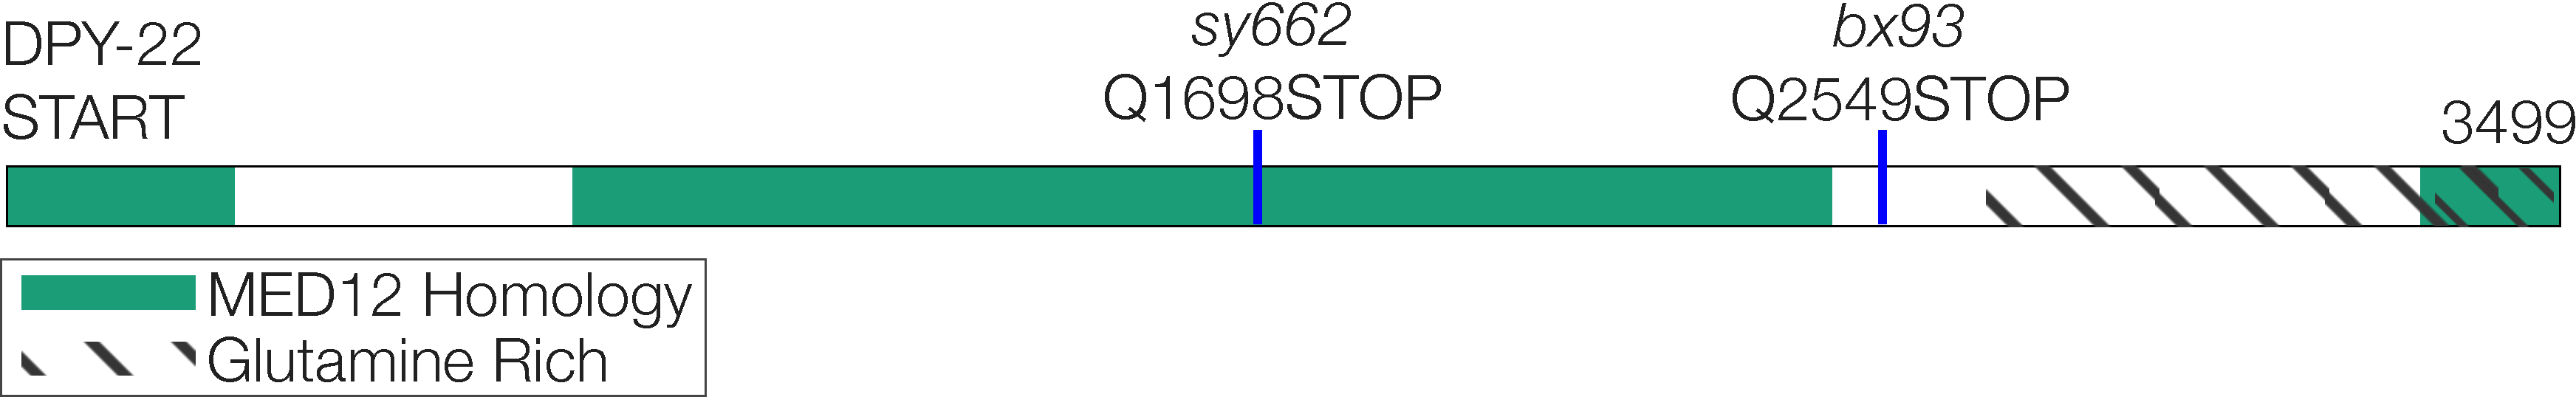
\includegraphics[width=0.5\textwidth]{../figs/Gene_Model.pdf}
  \caption{
           Protein sequence schematic for \protein{dpy-22}. The positions of the
           nonsense mutations used are shown.
           }
\label{fig:genemodel}
\end{figure}


\section*{Results and Discussion}
\subsection*{RNA-sequencing of three \gene{dpy-22} alleles and two known
             interactor genes}
We carried out RNA-seq on biological triplicates of mRNA extracted from \sy{}
homozygotes, \bx{} homozygotes and wild type controls, along with quadruplicates
from \emph{trans}-heterozygotes of both alleles with the genotype
\gene{dpy-6 dpy-22(bx93) / + dpy-22(sy622)}. We also sequenced mRNA
extracted from \gene{bar-1(ga80)} (a Wnt ortholog), \gene{let-60(n2021)} and
\gene{let-60(n1046gf)} (Ras ortholog) mutants in triplicate because these genes
have been previously described to interact with \dpy{} to form the
vulva~\cite{Moghal2003} and the male tail~\cite{Zhang2000}. Sequencing was
performed at a depth of 20 million reads per sample. Reads were pseudoaligned
using Kallisto~\cite{Bray2016}. We performed a differential expression using a
general linear model specified using Sleuth~\cite{Pimentel2016a}
(see~\nameref{sec:methods}). Differential expression with respect to the wild
type control for each transcript $i$ in a genotype $g$ is measured via a
coefficient $\beta_{g, i}$, which can be loosely interpreted as the natural
logarithm of the fold-change. Transcripts were considered to have differential
expression between wild-type and a mutant if the false discovery rate, $q$, was
less than or equal to 10\%. We used this method to identify the differentially
expressed genes associated with each mutant (see Table~\ref{tab:numbers};
\href{https://wormlabcaltech.github.io/med-cafe/notebook/basic.html}{Basic
Statistics Notebook})
Supplementary File 1 contains all the beta values associated with this project.
We have also generated a website containing complete details of all the analyses
available at the following URL:\@
\url{https://wormlabcaltech.github.io/med-cafe/analysis}.

\begin{table*}
 \centering
 \begin{tabular}{lc}
   \toprule
   Genotype & Differentially Expressed Genes\\
   \midrule
   \bx{} & \weakn{}\\
   \gene{dpy-6(e14)} \dpy{(bx93)} / \emph{+} \dpy{(sy622)} & \transn{}\\
   \sy{} & \strongn{}\\
   \gene{bar-1(ga80)} & 4613\\
   \gene{let-60(n2021)} & 509\\
   \gene{let-60(n1046gf)} & 2526\\
   \bottomrule
 \end{tabular}
 \caption{
          The number of differentially expressed genes relative to the wild-type
          control for each genotype with a significance threshold of 0.1
          }
\label{tab:numbers}
\end{table*}


\begin{figure}
  \centering{}
  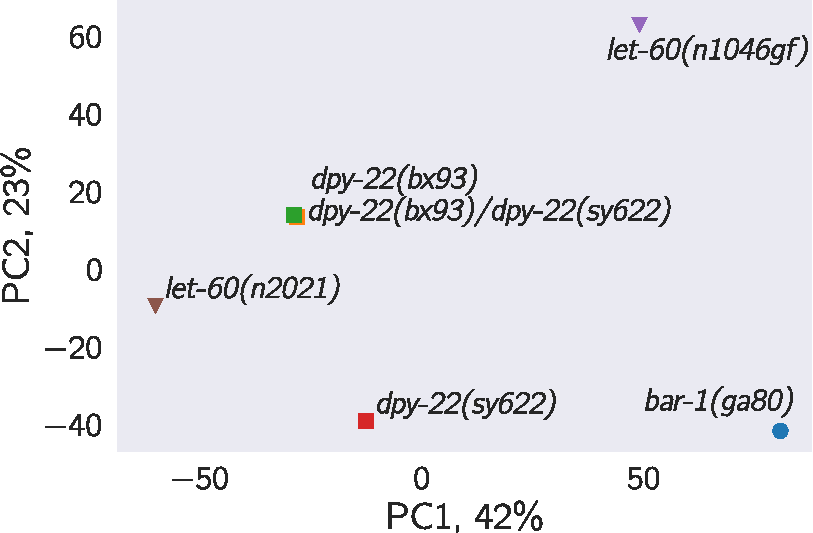
\includegraphics[width=0.5\textwidth]{../figs/pca.pdf}
  \caption{
           Principal component analysis of the analyzed genotypes. The
           analysis was performed using only those transcripts that were
           differentially expressed in at least one genotype. The plot shows
           that the \emph{trans}-heterozygotes phenocopy the \bx{} homozygotes
           along the first two principal dimensions.
           }
\label{fig:pca}
\end{figure}

\subsection*{Principal component analysis visualizes the allelic dominance of
             the \bx{} allele over \sy{}}
As a first step in our analysis, we performed dimensionality reduction on the
transcriptomes we sequenced using Principal Component Analysis (PCA). Briefly,
PCA identifies the vectors along which there is most variation in the data.
These vectors can be used to project the data into lower dimensions to assess
whether samples cluster, though interpreting the biological reasons for this
clustering can be challenging. To perform PCA, we selected only those
transcripts that were differentially in at least one genotype, and used the
$\beta$ coefficients associated with these genes to perform PCA.\@ Projecting
the data into two dimensions maintains 65\% of the variation. The first
dimension separates the gain and loss of function \gene{let-60} mutants. The
second dimension separates the \dpy{} mutants (see Fig.~\ref{fig:pca}). On the
PCA plot, the \emph{trans}-heterozygote mutants appear to phenocopy the \bx{}
mutants, recapitulating previous experiments that showed the \bx{} allele to be
dominant over the \sy{} allele.

\subsection*{Three \dpy{} genotypes have shared transcriptomic
             phenotypes}
Although the two dimensional PCA plot suggests strongly that the \bx{} allele is
dominant over the \sy{} allele, we would like to understand the degree and
nature of the dominance that is occurring. To construct a severity and dominance
hierarchy, we must establish how many transcriptomic phenotypes are
represented among the three \dpy{} genotypes, and of those phenotypes, how many
of them are shared transcriptomic phenotypes (STPs). Shared transcriptomic
phenotypes are defined as the set of genes that are commonly differentially
expressed in two mutant genotypes relative to a wild-type control, regardless
of the direction of change, as defined previously~\cite{AngelesAlboresHIF}. We
use the term in the plural version, because the shared genes may represent
multiple independent modules that formally constitute different phenotypic
classes.

We identified significant pairwise STPs between all \dpy{} mutants. The
transcripts that were differentially expressed in \bx{} homozygotes were almost
all differentially expressed in \sy{} homozygotes (189/\weakn{}) and in
\emph{trans}-heterozygotes (192/\weakn{}). On the other hand, although \sy{}
homozygotes and \emph{trans}-heterozygotes exhibited a similar number of
differentially expressed genes, less than half of these were shared between the
two genotypes.

\subsection*{False hit analysis identifies four non-overlapping phenotypic
             classes}

\begin{figure*}
 \centering{}
 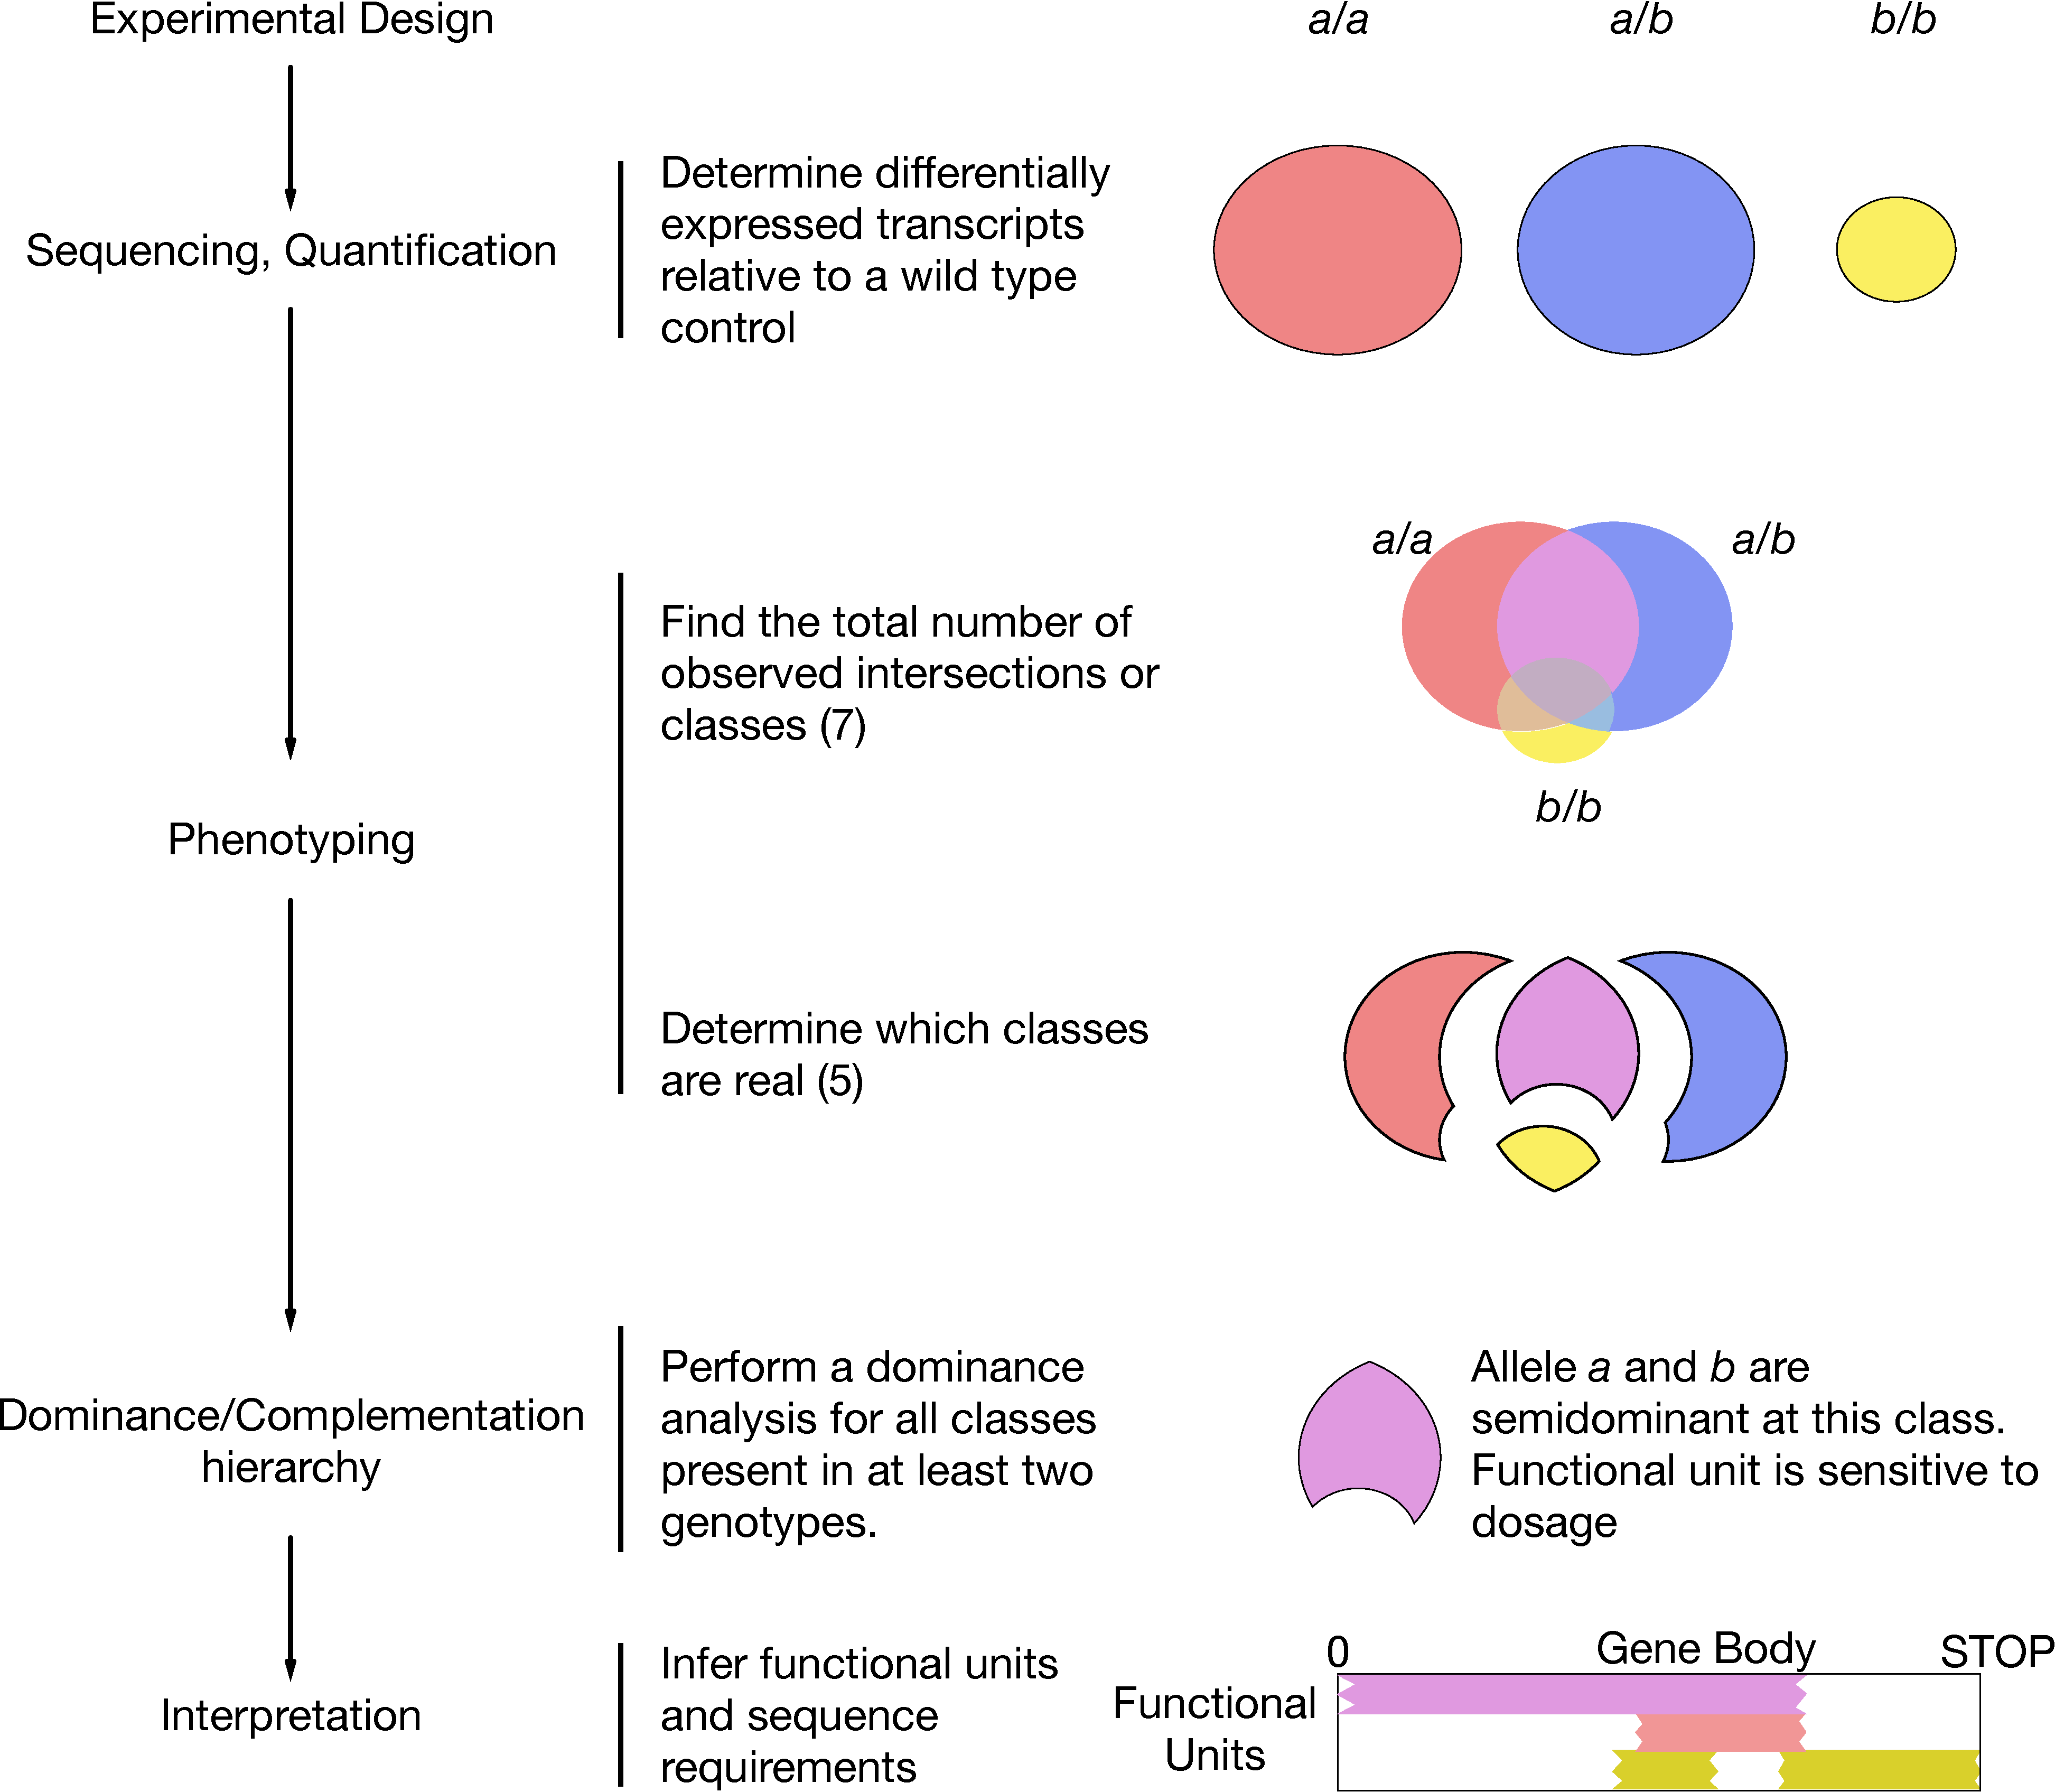
\includegraphics[width=\textwidth]{../figs/flowchart.pdf}
 \caption{
         Flowchart for an analysis of arbitrary allelic series. A set of alleles
         is selected, and the corresponding genotypes are sequenced. Independent
         phenotypic classes are then identified. For each phenotypic class, the
         alleles are ordered in a dominance/complementation hierarchy, which can
         then be used to infer functional regions within the genes in question.
         }
\label{fig:flowchart}
\end{figure*}

Severity and dominance hierarchies must be calculated with respect to each
independent phenotype associated with the alleles under study. A challenge with
expression profiles is to identify these independent phenotypes. We reasoned
that comparing the expression profiles of the two \dpy{} homozygotes and the
\emph{trans}-heterozygote would naturally partition the expression profiles into
groups that would constitute phenotypic classes. However, a three-way comparison
can give rise to 7 ($2^3$) possible groupings: transcripts perturbed in only a
single genotype (3), transcripts perturbed in two genotypes (3) and transcripts
perturbed in all three genotypes (1). A shortcoming of RNA-seq is that it is
prone to false positive and false negative artifacts, and these artifacts could
be numerous enough to cause the appearance of certain groups that would not
be there otherwise. In other words, we might find a subset of genes that are
differentially expressed in a single genotype, but if this subset is small
enough, we ought to be concerned that this subset is caused by false positive
hits within this genotype or false negative hits in the other genotypes. This
thought experiment highlights the need to assess which groups have sufficient
statistical support to consider as phenotypic classes.

We developed a method to assess whether groups in a Venn diagram are likely to
be the result of statistical artifacts. Briefly, the algorithm works by assuming
all of the data is the result of false positive and false negative hits except
for the group of transcripts that is differentially expressed in the maximum
number of genotypes. Then, using estimates for the false positive and negative
response, we calculate the expected sizes of all the groups after adding noise
under this model. If an observed group is much larger than expected by noise, we
refine the data model to accept the group. After accepting new groups into the
model, we calculate the noise again, and refine the model once more. This
process continues until the model converges. We called this method a false hit
analysis.

We used false hit analysis to identify four non-overlapping phenotypic classes.
We use the term genotype-specific to refer to groups of transcripts that were
perturbed in one mutant. We use the term genotype-associated to refer to those
groups of transcripts whose expression was significantly altered in two or more
mutants with respect to the wild type control. The \textbf{\sy{}-associated}
phenotypic class consisted of 720 genes differentially expressed in \sy{}
homozygotes and in \emph{trans}-heterozygotes, but which had wild-type
expression in \bx{} homozygotes. The \textbf{\bx{}-associated} phenotypic class
contains 403 genes differentially expressed in all genotypes. The
\bx{}-associated class included re-classified transcripts that had been found to
be differentially expressed in the \bx{} homozygote and one other genotype,
because these were very likely to be the result of false negative hits in the
missing genotype, and re-classifying these transcripts improved our model
substantially. We also identified a \textbf{\sy{}-specific} phenotypic class
(1,841 genes) and a \textbf{\emph{trans}-heterozygote-specific} phenotypic class
(1,226 genes; see the
\href{https://wormlabcaltech.github.io/med-cafe/notebook/phenotypic_classes.html}{
Phenotypic Classes Notebook}).

\subsection*{Severity hierarchy of a \gene{dpy-22} allelic series}
Having separated the expression profiles into phenotypic classes, we can ask
what the severity hierarchy is between the \bx{} allele and the \sy{} allele.
Broadly speaking, there are two ways to assess severity. First, we can ask which
allele affects causes more mutant phenotypes or phenotypic groups as a
homozygote (allelic pleiotropy). Alternatively, we can identify the allele which
causes the greatest change in expression in a homozygote at each shared
phenotype among the homozygotes of both alleles, which we refer to as
\textbf{allelic volume}\footnote{We chose the term volume by analogy with a
radio. Each allele can affect a different number of phenotypes (channels) with a
different perturbation magnitude per channel (volume)}. An important caveat is
that volume only makes sense if the homozygotes of each allele are well
correlated (i.e., they have a linear relationship with small spread). If the
phenotypes have zero or negative correlation between two homozygotes, then the
two alleles under inspection are not of the same kind, i.e., they cannot both be
loss-of-function alleles, or gain-of-function alleles for this phenotype.

The \sy{} homozygote shows more differentially expressed genes that participate
in a greater number of phenotypic classes relative to the \bx{} homozygote.
Thus, the \sy{} allele is a more pleiotropic mutation than the \bx{} allele. To
assess which allele has more volume,  Since the homozygotes of each allele only
share a single phenotypic class in common, we need only assess volume along
this single phenotype. To calculate a volume coefficient, for genes in the
\bx{}-associated phenotypic class, we plotted the $\beta$ coefficients from the
\sy{} homozygote against the $\beta$ coefficients from the \bx{} homozygote (see
Fig.~\ref{fig:stp}) and performed a linear regression to find the slope of this
line. Using this method, we found that the \bx{} homozygote has a volume that
is 60\% of the \sy{} homozygote. Taken together, these results suggest that the
\sy{} allele represents a more severe alteration-of-function mutation than the
mutation within the \bx{} allele. Moreover, within their shared phenotype, the
\bx{} allele encodes functionality that is more similar to wild-type than the
functionality encoded in the \sy{} allele.

\begin{figure}
  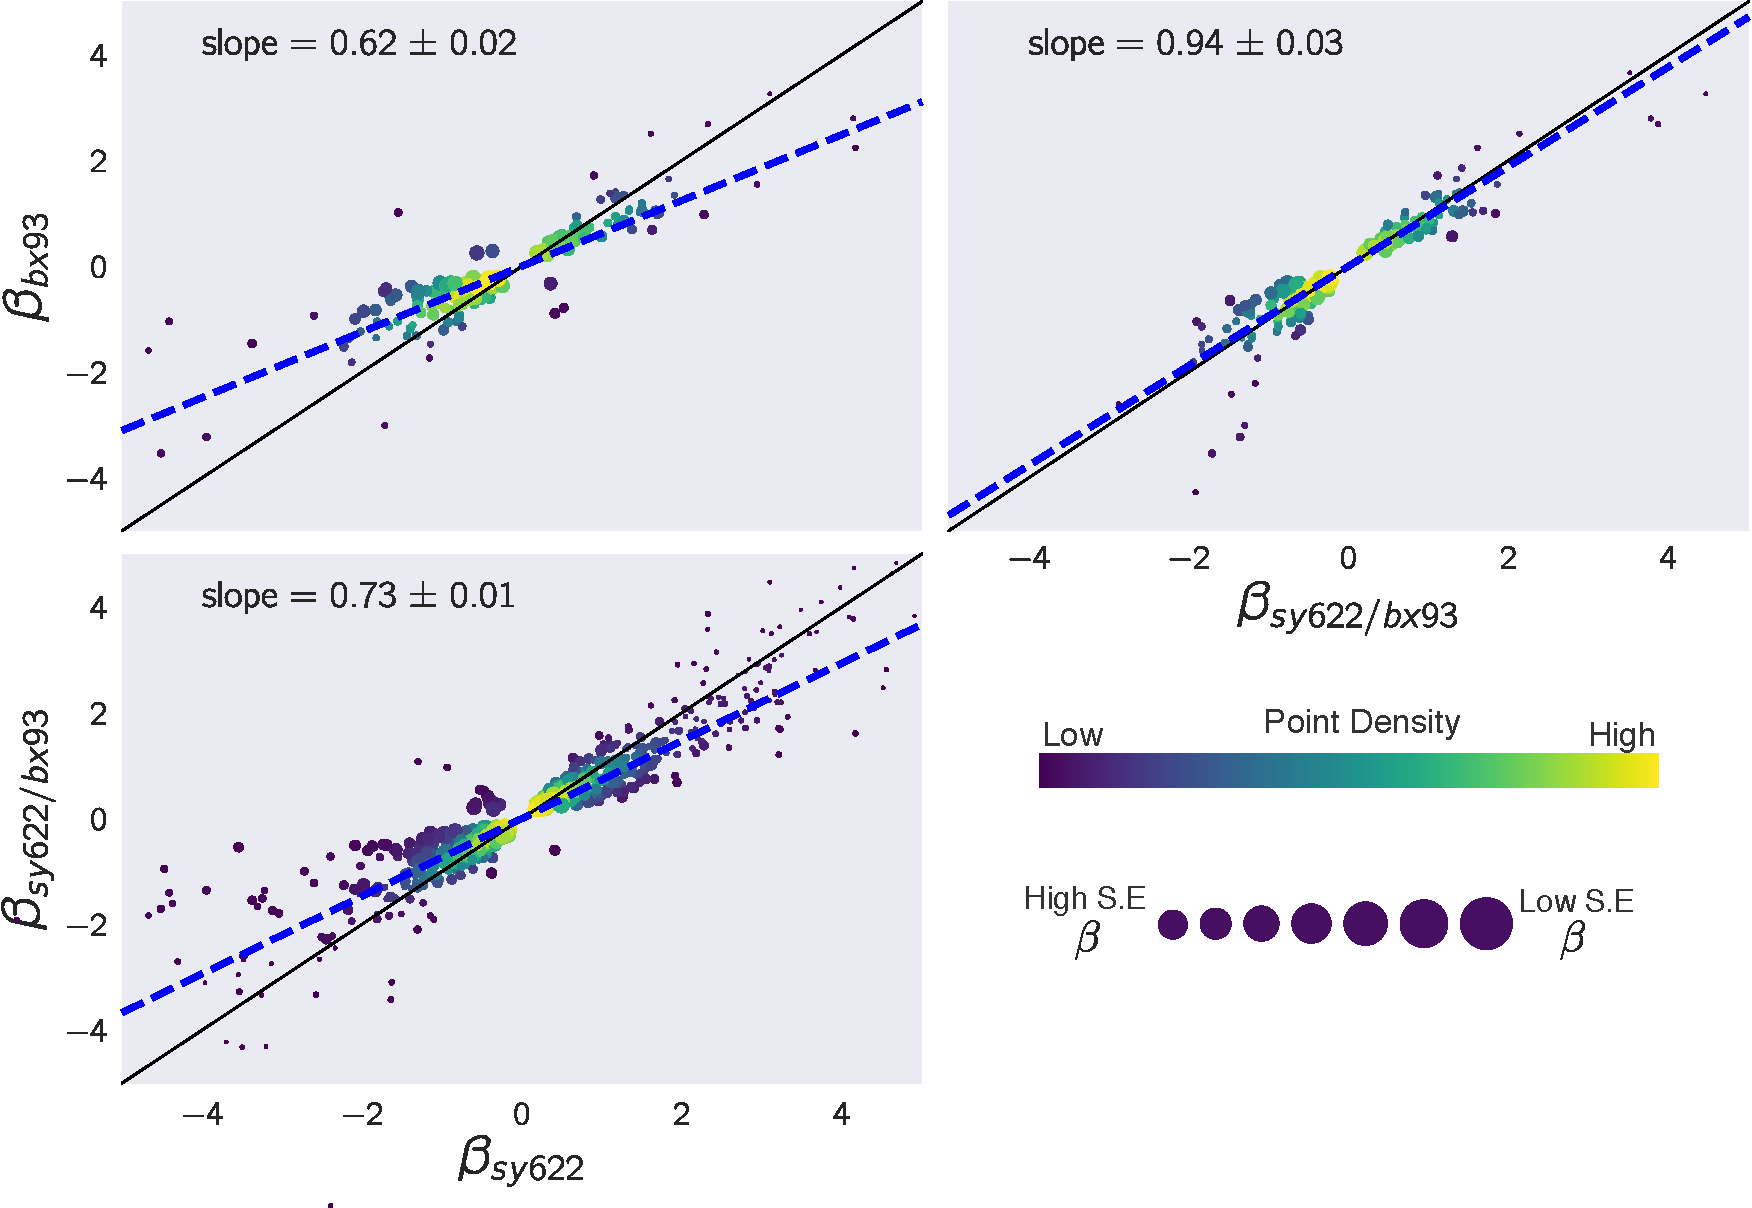
\includegraphics[width=0.5\textwidth]{../figs/dpy22-stps.pdf}
  \caption{
           Shared Transcriptomic Phenotypes amongst the \dpy{} genotypes are
           regulated in the same direction. For each pairwise comparison, we
           found those transcripts that were commonly differentially expressed
           in both genotypes relative to the wild-type control and plotted the
           $\beta$ coefficients for each. We performed a linear regression on
           each plot to find the line of best fit (broken blue line). Only the
           comparison between \sy{} and \bx{} homozygotes was used to establish
           that the volume of the \sy{} allele is greater than the volume of
           the \bx{} allele. The other comparisons are shown for completeness.
          }
\label{fig:stp}
\end{figure}

\subsection*{Dominance hierarchy of a \gene{dpy-22} allelic series}
We measured allelic dominance for each class using a dominance coefficient
(see~\nameref{sec:methods}). The dominance coefficient is a measure of the
contribution of each allele to the total expression level in
\emph{trans}-heterozygotes. By definition, the \sy{} allele is completely
recessive to \bx{} for the \sy{}-specific phenotypic class. To determine the
dominance coefficient for the other phenotypic classes, we first selected the
transcripts within those classes, and asked what linear combination of the
homozygotic $\beta$ coefficients best approximated the $\beta$ coefficients of
the \emph{trans}-heterozygote, subject to the constraint that the sum of the
weights for the two homozygotes should be equal to unity. We solved this problem
by finding the maximum likelihood estimate for these weights. Using this method,
we found that the \sy{} and \bx{} alleles are semidominant ($d_{bx93} = 0.48$)
to each other for the \sy{}-associated phenotypic class. The \bx{} allele is
largely  dominant over the \sy{} allele ($d_{bx93}=0.82$; see
Table~\ref{tab:dom}) for the \bx{}-associated phenotypic class.

\begin{table}
  \centering
  \begin{tabular}{lc}
    \toprule
    Phenotypic Class & Dominance\\
    \midrule
    \sy{}-specific & $1.00\pm0.00$\\
    \sy{}-associated & $0.48\pm0.01$\\
    \bx{}-associated & $0.82\pm0.01$\\
    \bottomrule
    % \midrule{}
  \end{tabular}
  \caption{
           Dominance analysis for the \dpy{/MDT12} allelic series. Dominance
           values closer to 1 indicate \bx{} is dominant over \sy{}, whereas 0
           indicates \sy{} is dominant over \bx{}.
          }
\label{tab:dom}
\end{table}

\section*{Phenotypic classes reflect morphological phenotypes}
Having identified a set of phenotypic classes, we wanted to know whether
enrichment analysis of anatomical, phenotypic or gene ontology terms revealed
relevant physiological aspects underlying our data. To this end, we used the
WormBase Enrichment Suite~\cite{Angeles-Albores2016} to perform enrichment
analysis of each group.

We found that the \bx{}-associated phenotypic class was enriched in genes
involved in `immune system processes' (\qval{5}), and was enriched in genes that
are expressed in the `intestine' (\qval{4}). The \sy{}-associated class on the
other hand was enriched in genes expressed in the `cephalic sheath cell'
(\qval{4}). Using the Gene Ontology Enrichment Analysis, we found that the
\sy{}-associated class is enriched in histones and histone-like proteins (`DNA
packaging complex' \qval{3}) as well as genes involed in `immune system
processes' (\qval{5}). The \sy{}-specific class was enriched in genes that have
expression in the `intestine' (\qval{7}), `muscular system' (\qval{3}) and
`epithelial system' (\qval{2}). The genes in this class are known to cause
bacterial lawn avoidance when knocked down or knocked out (\qval{2}). Finally,
GO enrichment showed that the \sy{}-specific class is specifically enriched in
`structural constituents of cuticle' (\qval{12}), namely `collagen trimers'
(\qval{12}) and in genes involved in respiration (\qval{6}). This last result
recapitulates the fact that \sy{} homozygotes show a severe Dumpy phenotype. The
\emph{trans}-heterozygote specific class was enriched in genes expressed in
`male' animals (\qval{63}) and genes expressed in the `reproductive system'
(\qval{21}). GO enrichment of genes in the \emph{trans}-heterozygote specific
class showed enrichment of the genes involved in the `regulation of cell shape'
(\qval{6}) and in a variety of terms involving phosphate metabolism, such as
`nucleoside phosphate binding' (\qval{5}), `dephosphorylation' (\qval{3}) or
`phosphorylation' (\qval{2}), suggesting that this class may be enriched in
genes involved in signal transduction though the reason for this enrichment
remains unclear. The \bx{}-specific class did not show enrichment on any test,
consistent with our interpretation that this class is the result of random false
positive hits.

\section*{Predicted interactions of Mediator with Wnt and Ras pathways in
          \cel{}}
Previous work in \cel{}~\cite{Moghal2003,Zhang2000} has implicated \dpy{} as an
inhibitor of the Wnt and Ras pathways during the formation of the vulva and the
male tail. We obtained expression profiles for \gene{bar-1(ga80)} mutants as
well as loss-of-function and gain-of-function Ras mutants, \gene{let-60(n2021)}
and \gene{let-60(n1046gf)} respectively. We predicted that the \sy{}-specific
phenotypic class would exhibit the most significant overlap (assessed by a
hypergeometric enrichment test) with differentially expressed genes in
\gene{let-60(n1046gf)} mutants, whereas the \bx{}-specific phenotypic class
would exhibit the most significant overlap with \gene{bar-1(ga80)} mutants.

There was no significant overlap between any of the mutants we tested and the
genes in the \bx{}-specific class, consistent with our interpretation of this
class as the result of random false positives (see Fig.~\ref{fig:wnt_stps}). All
other classes showed significant enrichment with genes perturbed in
\gene{bar-1(ga80)}. Similarly, \gene{let-60(n2021)} showed enrichment in all
real phenotypic classes, with the exception of the \emph{trans}-heterozygote
specific class. Contrary to our hypotheses, differentially expressed genes in
\gene{let-60(n1046gf)} did not show significant overlap with the \sy{}-specific
phenotype, but they did show significant overlap with all remaining real
phenotypic classes.

\begin{figure}
  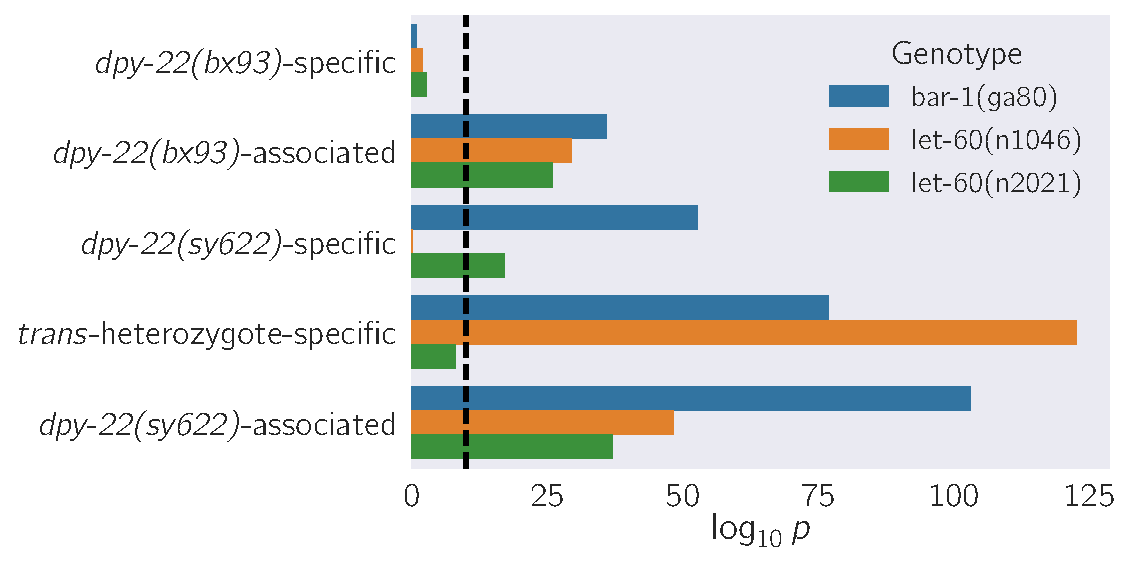
\includegraphics[width=0.5\textwidth]{../figs/stp_pvals.pdf}
  \caption{
          \dpy{} phenotypic classes are statistically significantly enriched
          for signatures of \gene{let-60} (ras) and \gene{bar-1} (wnt)
          signaling.
          We tested whether the overlap between the differentially expressed
          genes in \gene{bar-1(ga80)}, \gene{let-60(n1046gf)} or
          \gene{let-60(n20201)} and the \dpy{} phenotypic classes was
          statistically significant using a hypergeometric enrichment test.
          Since the hypergeometric enrichment test is very sensitive to
          deviations from random, and since we suspect that there may be a broad
          genotoxic response to all mutants, we used a statistical significance
          threshold of $p < 10^{-10}$ (dashed black line).
  }
\label{fig:wnt_stps}
\end{figure}

\section*{Discussion}
\label{sec:conclusions}
\subsection*{Phenotypic classes and their sequence requirements}
Because the mutations we used are truncations, our results suggest the existence
of various functional regions in \dpy{/MDT12} (see Fig.~\ref{fig:domains}).
These functional regions could encode protein domains with biochemical activity,
or they could encode biochemically active amino acid motifs, such as nuclear
localization sequences or protein binding sites. The \sy{}-specific phenotypic
class is likely controlled by a single functional region, functional region 1
(FR1). Sequence necessary for wild-type FR1 functionality is encoded between
amino acid positions 0 and 2,549. The \sy{}-associated phenotypic class is
likely controlled by a second functional region, functional region 2 (FR2), and
some necessary sequences for wild-type function are encoded between
amino acid positions 1,698 and 2,549. We speculate that this functional region
may be the reason that \emph{bx93} is unable to complement the Muv phenotype of
\emph{sy622} in a sensitized \emph{let-23} background, since
\emph{trans}-heterozygotes in this background exhibit a semidominant Muv
phenotype. It is unlikely that FR1 and FR2 are identical because their dominance
behaviors are very different. The \bx{} allele was largely dominant over the
\sy{} allele for the \bx{}-associated class, but gene expression in this class
was perturbed in both homozygotes. The perturbations were greater for \sy{}
homozygotes than for \bx{} homozygotes. This behavior can be explained if the
\bx{}-associated class is controlled jointly by two distinct effectors,
functional regions 3 and 4 (FR3, FR4, see Fig.~\ref{fig:domains}). Such a model
would propose that the sequences necessary for FR3 functionality are within the
interval 0 and 1,698, and some sequences necessary for FR4 functionality are
encoded between positions 2549 and 3499. This model explains how expression
levels of the \emph{bx93}-associated phenotypic class in the
\emph{trans}-heterozygote are complemented to the levels of the \emph{bx93}
homozygote, because FR3 is complemented in \emph{trans}, but FR4 is defective.
Thus, FR3 encodes a functionality that is not dosage-dependent. One possibility
is that FR3 is equivalent to FR2, and FR4 modifies its activity at a subset of
loci. A rigorous examination of this model will require studying many alleles
that mutate the region between Q1689 and Q2549 using homozygotes and
\emph{trans}-heterozygotes.

\begin{figure}
  \centering{}
  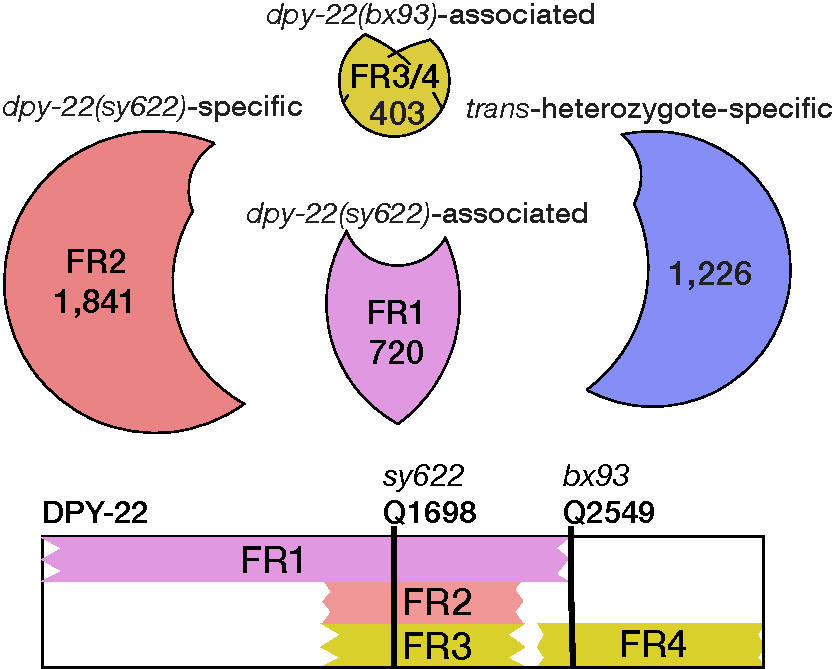
\includegraphics[width=0.5\textwidth]{../figs/inferred_domains.pdf}
  \caption{
          The functional regions associated with each phenotypic class can be
          mapped intragenically. The number of genes associated with each class
          is shown. The \bx{}-associated class may be controlled by two
          functional regions. FR2 and FR3 could be redundant if FR4 is a
          modifier of FR2 functionality at \bx{}-associated loci. Note that the
          \bx{}-associated phenotypic class is actually three classes merged
          together. Two of these classes are DE in \bx{} homozygotes and one
          other genotype. Our analyses suggested that these two classes are
          likely the result of false negative hits and genes in these classes
          should be differentially expressed in all three genotypes, so we
          merged these three classes together (see~\nameref{sec:methods}).
  }
\label{fig:domains}
\end{figure}

We also found a class of transcripts that had perturbed levels in
\emph{trans}-heterozygotes only; its biological significance is unclear.
Phenotypes unique to \emph{trans}-heterozygotes are often the result of physical
interactions such as homodimerization, or dosage reduction of a toxic
product~\cite{Yook2005}. In the case of \dpy{/MDT12} orthologs, how either
mechanism could operate is not obvious, since \protein{dpy-22} is expected to
assemble in a monomeric manner into the CKM.\@ Massive single-cell RNA-seq of
\cel{} has recently been reported~\cite{Cao2017}. When this technique becomes
cost-efficient, single-cell profiling of these genotypes may provide information
that complements the whole-organism expression phenotypes, perhaps explaining
the origin of this phenotype.

\subsection*{Phenotypes, not molecular pathways}
In an attempt to better dissect interactions between \dpy{} and \gene{let-60}
(ras) and \gene{bar-1} (wnt), we obtained expression profiles of these mutants
and looked for enrichment within each phenotypic class. Prior research suggested
that the \emph{bx93}-associated class should show STPs with \gene{bar-1} mutant
transcriptomes but not with \gene{let-60} mutant transcriptomes, and the
\emph{sy622}-specific class should show STPs with gain-of-function \gene{let-60}
mutants but not with \gene{bar-1} null mutants. Instead, we found that
\gene{let-60} and \gene{bar-1} loss-of-function mutants had STPs with all the
phenotypic classes; and \gene{let-60} gain-of-function mutants did not show STPs
with the \emph{sy622}-associated class. Thus, although we could predict that
both of these genes are interactors with \dpy{}, our experiments did not enable
us to predict what functional regions mediate this interaction.

Our failure to predict what functional regions mediate interactions with other
pathways or to predict the valence of the interactions reflects the fact that we
are treating expression profiles as phenotypes, and not as a method to read out
the activity of molecular pathways. Expression profiles as phenotypes have
advantages, namely that they can be used for genetic analyses, but they also
come with disadvantages. In our case, we sequenced animals after development had
occurred, so the expression levels we observe are the average expression levels
of all tissues after they have finished forming. Moreover, as with any other
phenotype, we cannot discriminate between proximal or direct effects on gene
expression from second order or ripple effects. As with morphological
phenotypes, it may turn out to be the case that expression profiles, like any
other phenotype, will often reflect a limited number of phenotypic classes. In
some cases, these phenotypic classes may be associated with a molecular pathway
by the use of index sets generated from mutants in these pathways. In other
cases, they may reflect stresses and insults that the animals are suffering as a
result of suboptimal activity. The difference between these two classes matters,
since the conclusions that can be drawn from studying each one vary in their
scopes; however, it seems reasonable likely that both will prove useful.

\subsection*{Occam's razor}
Transcriptomic phenotypes generate large amounts of differential gene expression
data, so false positive and false negative rates can lead to spurious phenotypic
classes whose putative biological significance is badly misleading. Such
artifacts are particularly likely for small phenotypic classes, which should be
viewed with skepticism. Notably, errors of interpretation cannot be avoided by
setting a more stringent $q$-value cut-off: doing so will decrease the false
positive rate, but increase the false negative rate, which will in turn produce
smaller phenotypic classes than expected. Our method tries to avoid this pitfall
by using total error rate estimates to assess the plausibility of each class.
These conclusions are of broad significance to research where highly multiplexed
measurements are compared to identify similarities and differences in the
genome-wide behavior of a single variable under multiple conditions.

We have shown that transcriptomes can be used to study allelic series in the
context of a large, pleiotropic gene. We identified separable phenotypic classes
that would otherwise be obscured by other methods, correlated each class to a
functional region, and identified sequence requirements for each region. Given
the importance of allelic series for characterizing gene function and their
roles in specific genetic pathways, we are optimistic that this method will be a
useful addition to the geneticist's arsenal.

\section*{Methods}
\label{sec:methods}

\subsection*{Strains used}
Strains used were N2 wild-type (Bristol)~\cite{Brenner1974},
PS4087 \sy{}~\cite{Moghal2003},
PS4187 \bx{}~\cite{Zhang2000},
%line break inserted below because \gene{...} doesn't linebreak well
PS4176\\ \gene{dpy-6(e14) dpy-22(bx93)/ + dpy-22(sy622)}~\cite{Moghal2003},
MT4866 \gene{let-60(n2021)}~\cite{Beitel1990a},
MT2124 \gene{let-60(n1046gf)}~\cite{Beitel1990a} and
EW15 \gene{bar-1(ga80)}~\cite{Eisenmann1998}.
Lines were grown on standard nematode growth media (NGM) Petri plates seeded
with OP50 \ecol{} at 20\degree{}C~\cite{Brenner1974}.

\subsection*{Strain synchronization, harvesting and RNA sequencing}
With the exception of strain MT4866, strains were synchronized by bleaching
P$_0$'s into virgin S. basal (no cholesterol or ethanol added) for 8--12 hours.
Arrested L1 larvae were placed in NGM plates seeded with OP50 at 20\degree{}C
and grown to the young adult stage (assessed by vulval morphology and lack of
embryos). We discovered that MT4866 dies upon L1 starvation for this period of
time. As a result, we synchronized this strain by double bleaching~\cite{}.
Animals were picked if they were young adults, regardless of whether any vulval
or morphological phenotypes were present. RNA extraction and sequencing was
performed as previously described by Angeles-Albores \emph{et
al}~\cite{AngelesAlboresHIF, Angeles-Albores2017}. Briefly, young adults were
placed in 10$\mu$L of TE buffer,  and digested using  Recombinant Proteinase K
PCR Grade (Roche Lot 656 No. 03115 838001) incubated with 1\% SDS 657 and
1.25~$\mu$L RNA Secure (Ambion AM7005). Total RNA was extracted using the Zymo
Research Directzol RNA MicroPrep Kit (Zymo Research, SKU R2061).\@ mRNA was
subsequently purified using a NEBNext Poly(A) mRNA Magnetic Isolation Module
(New England Biolabs, NEB, \#E7490). Sequencing libraries were generated using
the NEBNext Ultra RNA Library Prep Kit for Illumina (NEB \#E7530). These
libraries were sequenced using an Illumina HiSeq2500 machine in single-read mode
with a read length of 50 nucleotides.

\subsection*{Read pseudo-alignment and differential expression}
Reads were pseudo-aligned to the \cel{} genome (WBcel235) using
Kallisto~\cite{Bray2016}, using 200 bootstraps and with the sequence bias
(\texttt{--seqBias}) flag. The fragment size for all libraries was set to 200
and the standard deviation to 40. Quality control was performed on a subset of
the reads using FastQC, RNAseQC, BowTie and
MultiQC~\cite{Andrews2010,Deluca2012,Langmead2009,Ewels2016}.

Differential expression analysis was performed using
Sleuth~\cite{Pimentel2016a}. We used a general linear model to identify genes
that were differentially expressed between wild-type and mutant libraries. To
increase our statistical power, we pooled young adult wild-type replicates from
other published~\cite{AngelesAlboresHIF,Angeles-Albores2017} and unpublished
analyses adjusting for batch effects. Briefly, batches were assigned based on
the a covariate that represented the combination of the person who collected the
worms, the person who extracted the RNA, the month in which the samples were
sequenced and the library preparation method.

\subsection*{False hit analysis}
To accurately count phenotypes, we developed a false hit algorithm
(Algorithm~\ref{alg:false}). We implemented this algorithm for three-way
comparisons in Python. Although experimentally restricted, a three-way
comparison can result in $128$ possible sets (ignoring size). This large number
of models necessitates an algorithmic approach that can at least restrict the
possible number of models. Our algorithm uses a noise function that assumes
false hit events are non-overlapping (i.e.\ the same gene cannot be the result
of two false positive events in two or more genotypes) to determine the average
noise flux between phenotypic classes. These assumptions break down rapidly if
false-positive or negative rates exceed 25\%.

To benchmark our algorithm, we generated one thousand Venn diagrams at random.
For each Venn diagram, we calculated the average false positive and false
negative flux matrices. Then, we added noise to each phenotypic class in the
Venn diagram, assuming that fluxes were normally distributed with mean and
standard deviation equal to the flux coefficient calculated. We input the noised
Venn diagram into our false hit analysis and collected classification
statistics. For a given signal-to-noise cutoff, $\lambda$, classification
accuracy varied significantly with changes in the total error rate. In the
absence of false negative hits, false hit analysis can accurately identify
non-empty genotype-associated phenotypic classes, but identifying
genotype-specific classes becomes difficult if the experimental false positive
rate is high. On the other hand, even moderate false negative rates ($>10\%$)
rapidly degrade signal from genotype-associated classes. For classes that are
associated with three genotypes, an experimental false negative rate of 30\% is
enough on average to prevents this class from being observed.

We selected $\lambda=3$ because classification using this threshold was high
across a range of false positive and false negative combinations. A challenge to
applying this algorithm to our data is the fact that the false negative rate for
our experiment is unknown. Although there has been significant progress in
controlling and estimating false positive rates, we know of no such attempts for
false negative rates. It is unlikely that the false negative rate for our study
is lower than the false positive rate, because all genotypes except the controls
are likely underpowered. We used false negative rates between 10--20\% for false
hit analysis. When the false negative rate was set at 15\% or higher, the
algorithm converged on the same five classes shown above. For false negative
rates between 10--15\%, the algorithm output the same five classes, but also
accepted the (\sy{},\bx{})-associated class. We selected the model corresponding
to false negative rates of 15--20\% because this model had lower $\chi^2$ values
than the model selected with a false negative rate of 10--15\% (4,212 versus
100,650).

We asked whether re-classification of some classes into others could improve
model fit. We manually re-classified the (\sy{},\bx{})-associated and the (\bx,
\emph{trans-heterozygote})-associated classes into the \emph{bx93}-associated
class (which is associated with all genotypes), and we compared $\chi^2$
statistics between a re-classified reduced model ($\chi^2=72$) and a reduced
model ($\chi^2=130$). Based on the lower $\chi^2$ of the re-classified reduced
model, we concluded that it is the most likely model to given our data.

\begin{algorithm}[H]
\label{alg:false}
  \DontPrintSemicolon{}

  \KwData{$\mathbf{M}_{obs} =  \{N_l\}$, an observed set of classes, where each
  class is labelled by $l\in L$ and is of size $N_l$. $f_p, f_n$, the false
  positive and negative rates respectively. $\alpha$, the signal-to-noise
  threshold for acceptance of a class.}
  \KwResult{$\mathbf{M}_{reduced}$, a reduced model that fits the data.}
  \BlankLine{}
  \Begin{
    \emph{Define a minimal set to initialize the reduced model}\;
    $\mathbf{K} = \{\min_{l \in L} N_l\}$\;

    \emph{Refine the model until the model converges or iterations max out}\;
    $i \leftarrow 0$\;
    $\mathbf{K_{prev}} \leftarrow \emptyset$\;
    \While{$(i < i_{\max})~|~(\mathbf{K_{prev}} \neq \mathbf{K}$)}{
      $\mathbf{K_{prev}} \leftarrow \mathbf{K}$\;

      \emph{Define a noise function to estimate error flows in
            $\mathbf{K}$}\;
      $\mathbf{F} \leftarrow \textrm{noise}(\mathbf{K}, f_p, f_n)$\;

      \For{$l \in L$}{
          \emph{Calculate signal to noise for each labelled class}\;
          \emph{False negatives can result in $\lambda < 0$}\;
          $\lambda_l \leftarrow \mathbf{M}_{obs, l}/F_{l}$\;
          % \emph{Use classes with high $\lambda_l$ to refine the model}\;
              \If{$(\lambda > \alpha)~|~(\lambda < 0)$}{
                $\mathbf{K}_l \leftarrow \mathbf{M}_{obs, l}$\;
              } %if
          } % end for
        $i++$
    } % end while
  } % end begin

  \emph{Return the reduced model}\;
  $\mathbf{M}_{reduced} = \mathbf{K}$\;
  \Return{$\mathbf{M}_{reduced}$}\;
  \BlankLine{}\;
  \caption{
          False Hit Algorithm. Briefly, the algorithm initializes a reduced
          model with the phenotypic class or classes labelled by the largest
          number of genotypes. This reduced model is used to estimate noise
          fluxes, which in turn can be used to estimate a signal-to-noise metric
          between observed and modelled classes. Classes that exhibit a high
          signal-to-noise are incorporated into the reduced model.
  }
\end{algorithm}

\subsection*{Dominance analysis}
\label{subsec:dominance}
We modeled allelic dominance as a weighted average of allelic activity:
% our model proposed that $\beta$ coefficients of the heterozygote,
% $\beta_{a/b,i,\text{Pred}}$, could be modeled as a linear combination of the
% coefficients of each homozygote:
\begin{equation}
  \beta_{a/b,i,\text{Pred}}(d_a) = d_a\cdot \beta_{a/a,i} +
                                   (1-d_a)\cdot \beta_{b/b,i},
\end{equation}
where $\beta_{k/k, i}$ refers to the $\beta$ value of the $i$th isoform in a
genotype $k/k$, and $d_a$ is the dominance coefficient for allele $a$.

To find the parameters $d_a$ that maximized the probability of observing the
data, we found the parameter, $d_a$, that maximized the equation:
\begin{equation}
    P(d_a|D,H,I) \propto \prod_{i \in S}
                   \exp{-\frac{{(\beta_{a/b,i,\text{Obs}} -
                                \beta_{a/b,i,\text{Pred}}(d_a))}^2}{
                                2\sigma_i^2}}
\end{equation}
where $\beta_{a/b,i,\text{Obs}}$ was the coefficient associated with the $i$th
isoform in the \emph{trans}-het $a/b$ and $\sigma_i$ was the standard error of
the $i$th isoform in the \emph{trans}-heterozygote samples as output by
Kallisto. $S$ is the set of isoforms that participate in the regression (see
main text). This equation describes a linear regression which was solved
numerically.

\subsection*{Code}
Code was written in Jupyter notebooks~\cite{Perez2007} using the Python
programming language. The Numpy, pandas and scipy libraries were used for
computation~\cite{VanDerWalt2011,McKinney2011,Oliphant2007} and the matplotlib
and seaborn libraries were used for data visualization~\cite{Hunter2007,Waskom}.
Enrichment analyses were performed using the WormBase Enrichment
Suite~\cite{Angeles-Albores2016,Angeles-Albores2018}. For all enrichment
analyses, a $q$-value of less than $10^{-3}$ was considered statistically
significant. For gene ontology enrichment analysis, terms were considered
statistically significant only if they also showed an enrichment fold-change
greater than 2.

\subsection*{Data Availability}
Raw and processed reads were deposited in the Gene Expression Omnibus. Scripts
for the entire analysis can be found with version control in our Github
repository, \url{https://github.com/WormLabCaltech/med-cafe}. A user-friendly,
commented website containing the complete analyses can be found at
\url{https://wormlabcaltech.github.io/med-cafe/}. Raw reads and quantified
abundances for each sample were deposited at the NCBI Gene Expression Omnibus
(GEO)~\cite{Edgar2002} under the accession code GSE107523
(\url{https://www.ncbi.nlm.nih.gov/geo/query/acc.cgi?acc=GSE107523}).

\section*{Acknowledgements}
This work was supported by HHMI with whom PWS was an investigator, by the
Millard and Muriel Jacobs Genetics and Genomics Laboratory at California
Institute of Technology, and by the NIH grant U41 HG002223. This article would
not be possible without help from Dr.\ Igor Antoshechkin and Dr.\ Vijaya Kumar
who performed the library preparation and sequencing. Han Wang, Hillel Schwartz,
Erich Schwarz, and Carmie Puckett Robinson provided valuable input throughout
the project.

%This is where your bibliography is generated.
\bibliography{citations}
% \bibliographystyle{naturemag}
\bibliographystyle{genetics}

\end{document}
